\chapter{Технологический раздел}
\label{cha:impl}

В данном разделе описываются средства, используемые для разработки программного продукта, требования для функционирования ПО, описываются результаты тестирования программного продукта.

\section{Выбор средств разработки}

\subsection{Выбор языка программирования}

Для написания программного продукта используется язык Python, так как для него существует множество готовых решений для работы с нейронными сетями. Так же выбранный язык сочетает в себе возможности функционального, структурного и объектно-ориентированного подходов, что позволяет кратко описывать математические конструкции, необходимые для решения поставленной задачи. Так же для данного языка существует большое количество различных математических библиотек, упрощающие работу с комплексными числами, и библиотек для обработки цифровых сигналов.

\subsection{Выбор среды программирования и отладки}

В качестве среды разработки для языка Python была выбрана кроссплатформенная IDE PyCharm. Предоставляет средства для анализа кода, графический отладчик, инструмент для запуска юнит-тестов. На данный момент PyCharm является бесплатным для образовательных учреждений и проектов с открытым исходным кодом.

Выбор данной среды разработки обусловлен следующими предоставляемыми возможностями, упрощающими разработку приложения и способствующими повышению качества исходного кода:

\begin{itemize}
	\item статический анализ кода;
	\item встроенный отладчик;
	\item навигация по проекту и исходному коду;
	\item рефакторинг;
	\item поддержка систем контроля версий.
\end{itemize}

\subsection{Используемые библиотеки}

Для упрощения реализации математических операций используется библиотека NumPy. Для считывания и записи аудио-файлов, а так же обработки сигналов используется библиотека LibROSA. Для работы с нейронной сетью используется библиотека TensorFlow. Для создания интерфейса используется фреймворк PyQt, который является Python-версией C++ фреймворка Qt.

\section{Система контроля версий}

В процессе разработки программы использовалась система контроля версий
Git. Система контроля версий позволяет вносить в проект атомарные изменения, направленные на решения каких-либо задач. В случае обнаружения ошибок или из- менения требований, вне-сенные изменения можно отменить. Кроме того, с помощью системы контроля версий решается вопрос резервного копирования.

Особенности Git:

\begin{itemize}
	\item данная система контроля версий является децентрализованной, что позволяет иметь несколько независимых резервных копий проекта;
	\item поддерживается хостингом репозиториев GitLab;
	\item поддерживается средой разработки PyCharm;
	\item предоставляет широкие возможности для управления изменениями проекта и просмотра истории изменений.
\end{itemize}

\section{Требования к вычислительной системе}

Для запуска программы необходимо иметь установленный на ЭВМ интерпретатор для Python 3.6 с установленными библиотеками. 

Так как выбранный язык программирования является кроссплатформенным, то требований к использованию операционной системы нет.

Алгоритмы работают с большими объёмами комплексных данных, поэтому объём оперативной памяти компьютера не должен быть меньше 1 ГБ, желательна архитектура x64 (x86-64).

\section{Формат данных}

Входом и выходом программного продукта являются WAV-файлы. Формат WAVE имеет четкую структуру, описанную в \cite{wav}.

WAV -- формат файла-контейнера для хранения записи оцифрованного аудиопотока, в котором для кодирования амплитуды вы- деляется фиксированное число бит.

WAV-файл состоит из двух частей. Одна из них -- заголовок файла, другая -- область данных. В заголовке файла хранится информация о:

\begin{itemize}
	\item размере файла;
	\item количестве каналов;
	\item частоте дискретизации;
	\item количестве бит в сэмпле (глубине звучания).
\end{itemize}

Длина заголовка составляет 44 байта. Область данных представляет собой набор амплитуд. 

В программе используется информация о количестве каналов и частоте дискретизации, а также амплитуды.

\section{Диаграмма классов}

Разработанный программный комплекс имеет два режима работы: режим обучения и нормальный режим. Диаграммы классов представлены на рисунках \ref{imp:train} и \ref{imp:run-diagram} соответственно.

\begin{figure}
	\centering
	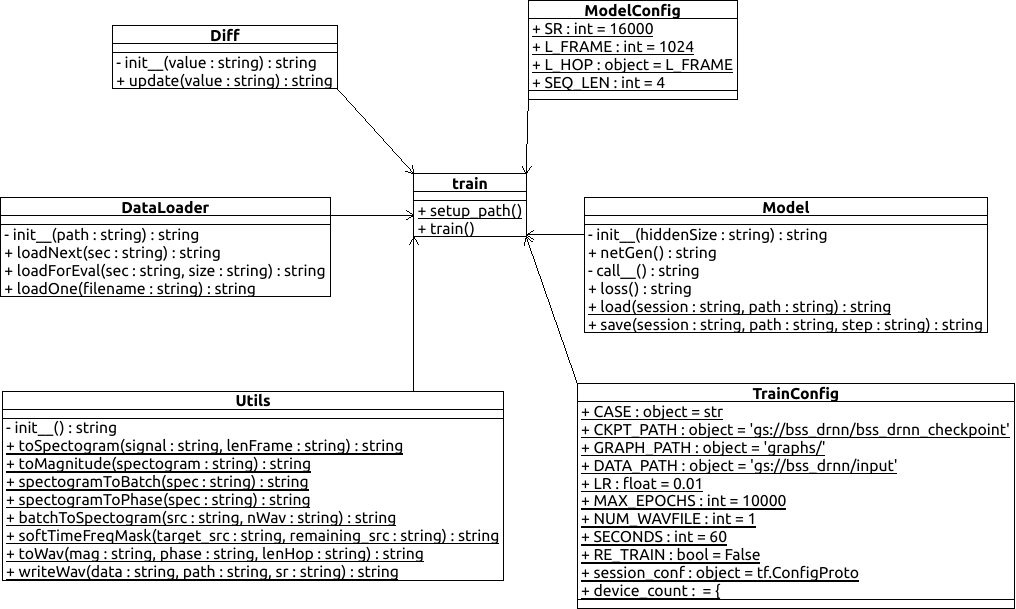
\includegraphics[width=\textwidth]{inc/img/train}
	\caption{Диаграмма классов программы нормального режима}
	\label{imp:train}
\end{figure}

\begin{figure}
	\centering
	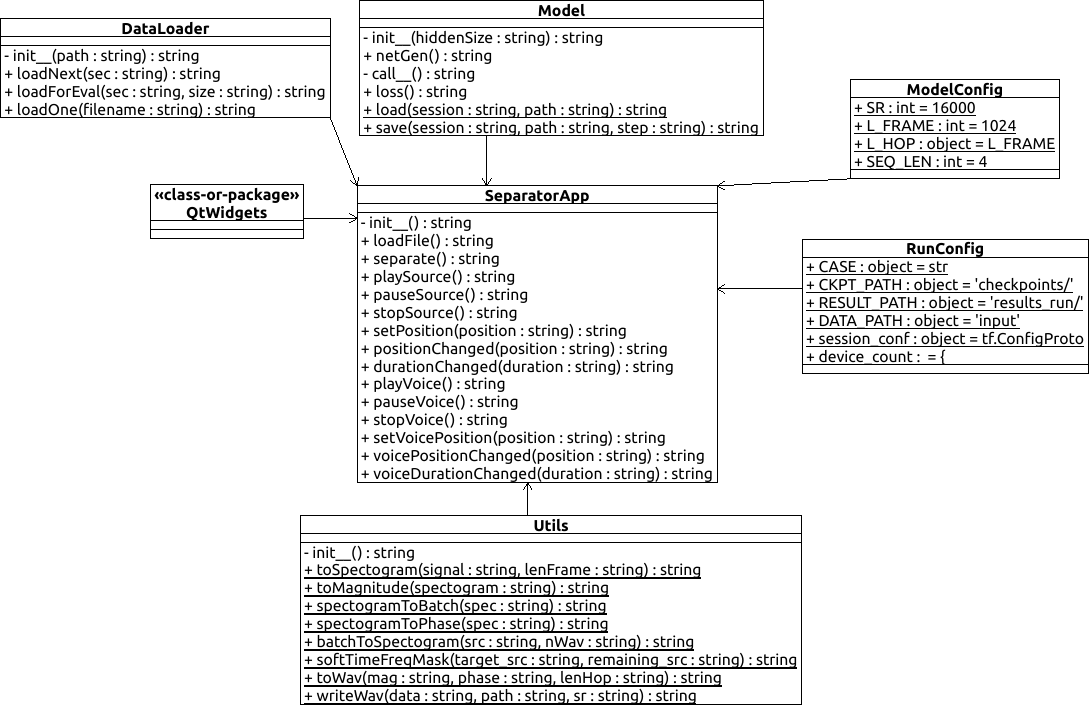
\includegraphics[width=\textwidth]{inc/img/run}
	\caption{Диаграмма классов программы нормального режима}
	\label{imp:run-diagram}
\end{figure}

\subsection{Описание классов}

\subsubsection*{DataLoader}

Отвечает за загрузку wav-файлов. Описание методов представлено в таблице \ref{imp:dataloader}.

\begin{table}[h]
	\caption{\label{imp:dataloader}Описание методов класса DataLoader}
	\begin{center}
		\begin{tabular}{|p{0.45\textwidth}|p{0.45\textwidth}|}
			\hline
			Метод & Описание \\
			\hline
			loadNext(sec) & Считывает очередной wav-файл из тренировочного набора данных, преобразуя его длину в sec \\
			\hline
			loadForEval(sec, size) & Считывает size случайных wav-файлов из тестового набора данных, преобразуя их длину в sec \\
			\hline
			loadOne(filename) & Считывает один файл с именем filename \\ 			
			\hline
		\end{tabular}
	\end{center}
\end{table} 

\subsubsection*{Diff}

Представляет ошибку, получаемую в процессе обучения и ее изменение. Описание методов представлено в таблице \ref{imp:diff}.

\begin{table}[h]
	\caption{\label{imp:diff}Описание методов класса Diff}
	\begin{center}
		\begin{tabular}{|p{0.45\textwidth}|p{0.45\textwidth}|}
			\hline
			Метод & Описание \\
			\hline
			update(sec) & Обновление значения ошибки и вычисление разницы с предыдущей ошибкой \\	
			\hline
		\end{tabular}
	\end{center}
\end{table} 

\subsubsection*{Model}

Представляет модель нейронной сети. Описание методов представлено в таблице \ref{imp:model}.

\begin{table}[h]
	\caption{\label{imp:model}Описание методов класса Model}
	\begin{center}
		\begin{tabular}{|p{0.45\textwidth}|p{0.45\textwidth}|}
			\hline
			Метод & Описание \\
			\hline
			load(session, path) & Загружает информацию об обученной модели для сессии sess из файлов сохранения, расположенных в path \\	
			\hline
			save(session, path) & Сохраняет информацию о модели из сессии sess в папку path \\
			\hline
			netGen() & Генерация нейронной сети \\
			\hline
		\end{tabular}
	\end{center}
\end{table} 

\subsubsection*{ModelConfig}

Представляет класс конфигурации для класса Model. Описание атрибутов представлено в таблице \ref{imp:modelconfig}.

\begin{table}[h]
	\caption{\label{imp:modelconfig}Описание методов класса Model}
	\begin{center}
		\begin{tabular}{|p{0.45\textwidth}|p{0.45\textwidth}|}
			\hline
			Атрибут & Описание \\
			\hline
			SR & Частота дискретизации wav-файла \\	
			\hline
			L\_FRAME & Размер окна в ОПФ \\
			\hline
			L\_HOP & Количество аудио кадров между столбцами ОПФ \\
			\hline
		\end{tabular}
	\end{center}
\end{table}

\subsubsection*{RunConfig}

Представляет класс конфигурации для класса SeparationApp. Описание атрибутов представлено в таблице \ref{imp:runconfig}.

\begin{table}[h]
	\caption{\label{imp:runconfig}Описание атрибутов класса RunConfig}
	\begin{center}
		\begin{tabular}{|p{0.45\textwidth}|p{0.45\textwidth}|}
			\hline
			Атрибут & Описание \\
			\hline
			CKPT\_PATH & Путь к файлам сохранения обученной модели \\	
			\hline
			RESULT\_PATH & Путь сохранения результата работы метода выделения \\
			\hline
			session\_conf & Конфигурация сессии tensorflow \\
			\hline
		\end{tabular}
	\end{center}
\end{table}

\subsubsection*{SeparationApp}

Представляет контроллер работы программы в нормальном режиме. Описание основных методов представлено в таблице \ref{imp:app}.

\begin{table}[h]
	\caption{\label{imp:app}Описание методов класса SeparationApp}
	\begin{center}
		\begin{tabular}{|p{0.45\textwidth}|p{0.45\textwidth}|}
			\hline
			Метод & Описание \\
			\hline
			loadFile() & Загрузка файла с помощью файлового менеджера \\	
			\hline
			separate() & Исполнение метода выделения источников \\
			\hline
		\end{tabular}
	\end{center}
\end{table} 

\subsubsection*{train}

Представляет контроллер работы программы в режиме обучения. Описание основных методов представлено в таблице \ref{imp:train-}.

\begin{table}[h]
	\caption{\label{imp:train-}Описание методов класса train}
	\begin{center}
		\begin{tabular}{|p{0.45\textwidth}|p{0.45\textwidth}|}
			\hline
			Метод & Описание \\
			\hline
			setup\_path() & Настройка путей для файлов сохранения \\	
			\hline
			train() & Обучение нейронной сети \\
			\hline
		\end{tabular}
	\end{center}
\end{table} 

\subsubsection*{TrainConfig}

Представляет класс конфигурации для класса train. Описание атрибутов представлено в таблице \ref{imp:trainconfig}.

\begin{table}[h]
	\caption{\label{imp:trainconfig}Описание атрибутов класса TrainConfig}
	\begin{center}
		\begin{tabular}{|p{0.45\textwidth}|p{0.45\textwidth}|}
			\hline
			Атрибут & Описание \\
			\hline
			CKPT\_PATH & Путь к файлам сохранения обученной модели \\	
			\hline
			GRAPH\_PATH & Путь к файлам сохранения инфографики процесса обучения \\	
			\hline
			DATA\_PATH & Путь к файлам обучающей выборки \\
			\hline
			LR & Коэффициент обучения \\
			\hline
			MAX\_EPOCHS & Количество эпох обучения \\
			\hline
			session\_conf & Конфигурация сессии tensorflow \\
			\hline
		\end{tabular}
	\end{center}
\end{table}

\subsubsection*{Utils}

Представляет вспомогательные функции. Описание методов представлено в таблице \ref{imp:utils}.

\begin{table}[h]
	\caption{\label{imp:utils}Описание методов класса Utils}
	\begin{center}
		\begin{tabular}{|p{0.45\textwidth}|p{0.45\textwidth}|}
			\hline
			Метод & Описание \\
			\hline
			toSpectogram(signal, lenFrame, lenHop) & Получение спектрограммы сигнала \\	
			\hline
			toMagnitude(spectogram) & Амплитудная составляющая спектрограммы \\
			\hline
			spectogramToPhase(spec) & Фазовая составляющая спектрограммы \\
			\hline
			toWav(mag, phase, lenHop) & Преобразование спектрограммы в сигнал \\
			\hline
			writeWav(data, path, sr) & Запись сигнала в аудио файл \\
			\hline
		\end{tabular}
	\end{center}
\end{table} 

\section{Построение нейронной сети}

В представлении Tensorflow нейронная сеть является графом потока данных, в котором данные в виде многомерного массива переходят в разные узлы, в процессе чего происходят все необходимые вычисления.

Каждое вычисление в TensorFlow представляется как граф потока данных. У него есть два элемента:

\begin{itemize}
	\item tf.Operation -- единицы вычислений.
	\item tf.Tensor -- представляет единицы данных (тенсоры).
\end{itemize}

Алгоритм \ref{imp:init-model} описывает инициализацию модели. Для определения входных и выходных данных используются тенсоры типа tf.placeholder. Плейсхолдер нужен исключительно в качестве цели наполнения. Он не инициализирован и не содержит данных.

\begin{minipage}{0.75\textwidth}
\begin{algorithm}[H]
\lstinputlisting[language=Python]{inc/src/model.py}
\caption{Исходный код инициализации модели}
\label{imp:init-model}
\end{algorithm}
\end{minipage}

Алгоритм \ref{imp:gen-model} описывает генерацию сети. Библиотека Tensorflow позволяет описывать граф многослойной рекуррентной нейронной сети с помощью встроенной функций tf.nn.dynamic\_rnn. В качестве параметра в функцию передается объект типа RNNCell.

Для описания графа обычных слоев используется функция tf.layers.dense.

\begin{minipage}{0.75\textwidth}
\begin{algorithm}[H]
	\lstinputlisting[language=Python]{inc/src/gen.py}
	\caption{Исходный код генерации сети}
	\label{imp:gen-model}
\end{algorithm}
\end{minipage}

Итоговый граф изображен на рисунке \ref{imp:graph}.

\begin{figure}
	\centering
	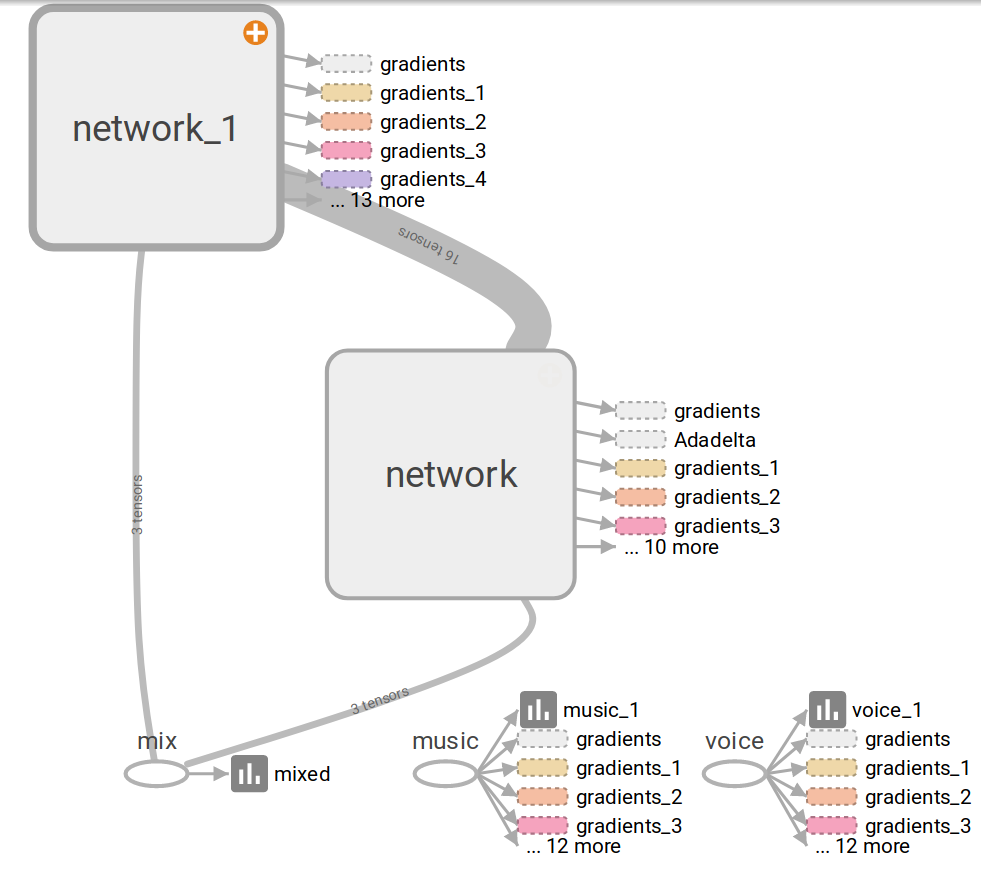
\includegraphics[width=0.7\textwidth]{inc/img/tensorboard-main}
	\caption{Граф модели}
	\label{imp:graph}
\end{figure}

\section{Установка программного обеспечения}

Для работы программного комплекса необходимо иметь на ПК интерпретатор для Python 3, установщик которого поставляется вместе с программным обеспечением. Для установки необходимых библиотек используется каталог программного обеспечения PyPI (Python Package Index). Все необходимые зависимости указаны в файле requirements.txt, благодаря чему установка библиотек выполняется одной командой:

\textbf{pip3 install -r requirements.txt}

\section{Руководство пользователя}

Разработанный программный комплекс имеет два режима работы: режим обучения и нормальный режим.

\subsection{Режим обучения}

Для обучения нейронной сети используется набор данных, путь до которых указывается в поле $DATA\_PATH$ класса конфигурации $TrainConfig$. Обучение происходит за $MAX\_EPOCHS$ эпох с коэффициентом обучения $LR$. За одну эпоху происходит обработка каждого WAV-файла из набора данных, после которых происходит корректировка весов.

Запуск обучения выполняется командой

\textbf{python3 train.py}

В процессе обучения генерируются вспомогательные файлы:
\begin{itemize}
	\item Файлы состояния сети, которые загружаются в последствии для установки обученных весов. Дирректория для хранения данных файлов задается параметром $CKPT\_PATH$.
	\item Файлы графиков процесса обучения. Задаются параметром $GRAPH\_PATH$. Для визуализации графиков используется утилита TensorBoard, которая входит в состав библиотеки TensorFlow. Для запуска утилиты используется команда:
	
	\textbf{tensorboard --logdir=/tmp/example/}
	
	где <</tmp/example/>> -- путь до сгенерированных файлов графиков. Данная команда запускает локальный сервер, для доступа к которому необходимо открыть в браузере адрес http://localhost:6006/.
	
	\item Файл журналирования обучения sample.log. В нем отражается информация о работе обучения, в том числе информация об изменении ошибки.
	
\end{itemize}
 
\subsection{Нормальный режим}

В нормальном режиме используется уже обученная нейронная сеть. Обученное состояние сети загружается из файлов, полученных во время обучения. Для удобства пользователя программное обеспечение поставляется вместе с файлами. Для запуска программы в нормальном режиме используется команда

\textbf{python3 run.py}

После запуска программы появляется главное окно (рисунок \ref{imp:main-window})

\begin{figure}
	\centering
	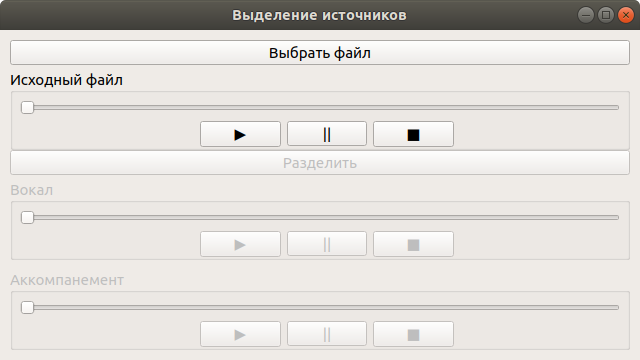
\includegraphics[width=0.8\textwidth]{inc/img/prog-main}
	\caption{Окно программы после запуска}
	\label{imp:main-window}
\end{figure}

На главном окне представлены следующие элементы:

\begin{enumerate}
	\item Кнопка <<Выбрать файл>>. Выводит окно выбора WAV-файла.
	\item Блок <<Исходный файл>>. Управляет воспроизведение исходного аудио файла. Состоит из следующих элементов:
	\begin{enumerate}
		\item Полоса прокрутки. Устанавливает момент воспроизведения, отображает процесс воспроизведения.
		\item Кнопки << $ \blacktriangleright $>>, <<||>>, <<$\blacksquare$ >> (начало воспроизведения, пауза и остановка воспроизведения соответственно). Управляют воспроизведением аудио файла.
	\end{enumerate}
	\item Кнопка <<Разделить>>. Инициализирует работу алгоритма выделения. После завершения работы метода активирует блоки <<Вокал>> и <<Аккомпанимент>> (рисунок \ref{imp:complete}).

	\item Блок <<Вокал>>. Управляет воспроизведением аудио файла голосовой составляющей. Функционал элементов соответствует блоку <<Исходный файл>>.
	\item Блок <<Аккомпанимент>>. Управляет воспроизведением аудио файла аккомпанимента. Функционал элементов соответствует блоку <<Исходный файл>>. 
\end{enumerate}


\begin{figure}
	\centering
	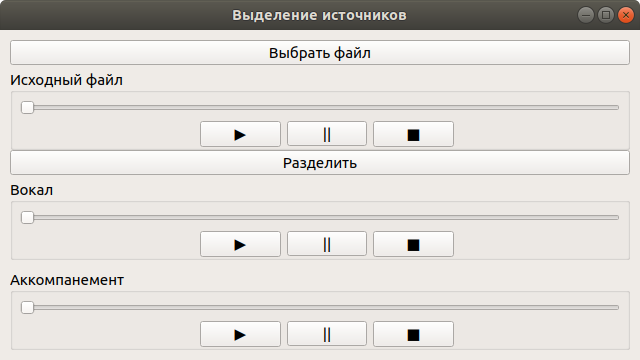
\includegraphics[width=0.8\textwidth]{inc/img/complete-window}
	\caption{Окно программы после работы метода выделения}
	\label{imp:complete}
\end{figure}

\section{Вывод}

На основе созданной архитектуры был разработан программный продукт на языке Python с использованием библиотек PyQt, TensorFlow, LibROSA и NumPy в среде PyCharm. Продукт был разработан на ЭВМ со следующими характеристиками:

\begin{itemize}
	\item Процессор: Intel Core i5.
	\item Частота процессора: 2.80GHz.
	\item Объем оперативной памяти: 8 Гб.
	\item Видеокарта: NVIDIA GeForce 840M.
	\item Операционная система: ubuntu 18.04 LTS.
\end{itemize}

Обучение нейронной сети происходило на удаленном ЭВМ со следующими характеристиками:

\begin{itemize}
	\item Количество процессоров: 2.
	\item Частота каждого из процессоров: 3.20GHz.
	\item Объем оперативной памяти: 2 Гб.
	\item Операционная система: ubuntu 16.04 LTS.
\end{itemize}

%%% Local Variables:
%%% mode: latex
%%% TeX-master: "rpz"
%%% End:
